\section{Antigen-escape constraint audit (gnomAD v4, HGNC, Reactome)}
\label{sec:constraint}
A CAR-T antigen is only as durable as the cost of losing it. CD19-negative relapse after CD19 CAR-T is the clinical precedent.
We asked what it costs a tumour to lose each gated antigen, on three orthogonal axes.
First, germline loss-of-function tolerance: gnomAD v4 LOEUF (the upper bound of the observed/expected LoF ratio; constrained when $<0.6$).
Second, paralog redundancy: HGNC gene-group size.
Third, pathway embedding: the number of Reactome pathways containing the protein.
\begin{equation}
\mathrm{LOEUF}(g) = \mathrm{upper\ CI}_{90}\!\left(\frac{\mathrm{obs\ LoF}_g}{\mathrm{exp\ LoF}_g}\right), \qquad \mathrm{LOEUF} < 0.6 \Rightarrow \text{LoF-intolerant}
\end{equation}
\paragraph{Calibration gate passes.} The four essential-gene controls (POLR2A, RPS3, PCNA, PSMA1) all read LoF-constrained (LOEUF 0.19-0.33; 4/4 below 0.6), so the gnomAD query and threshold behave before any claim is made.
\paragraph{Gate-wide null on all three escape-cost axes.} Gated antigens are not more LoF-tolerant than a random surfaceome background (median LOEUF 1.02 vs 0.95, Mann-Whitney $p=0.460$; constrained fraction 18/97 vs 16/72, Fisher $p=0.567$), not less paralog-redundant (median HGNC group size 18 vs 29, $p=0.073$), and if anything more pathway-embedded (median Reactome pathways 2 vs 1, $p=0.0005$).
The pathway-embedding difference survives the composition control (protein-coding, non-olfactory, non-IG/TCR loci only: $p=0.0096$), but it runs the safe direction for therapy: gated antigens sit in more curated biology, not less.
\paragraph{Every measurable AND-gate antigen is free to lose.} Combining germline tolerance with the committed DepMap 24Q4 CRISPR audit (fraction of 1,178 lines dependent $<0.1$), 6 of the seven AND-gate antigens land in the free-loss quadrant: CLDN18, CA9, CA12, MSLN, PSCA and SLC39A6 are all LoF-tolerant (LOEUF 1.01 or higher) and non-essential in every cancer line tested (max dependent fraction 3.1\%).
CLDN6 is unmeasurable for LOEUF (no gnomAD constraint row) and non-essential (3.1\%); it is recorded as unknown, not assumed constrained.
The approved references behave the same way (CD19, FOLR1, TNFRSF17 free-loss; ERBB2 doubly constrained by both germline and tumour dependency), so free-loss status is the norm for clinically used antigens rather than a defect of our gate; it means antigen heterogeneity and escape must be engineered around (AND-gating helps only if the partner antigen is co-expressed), not that the targets are wrong.
\begin{figure}[t]\centering
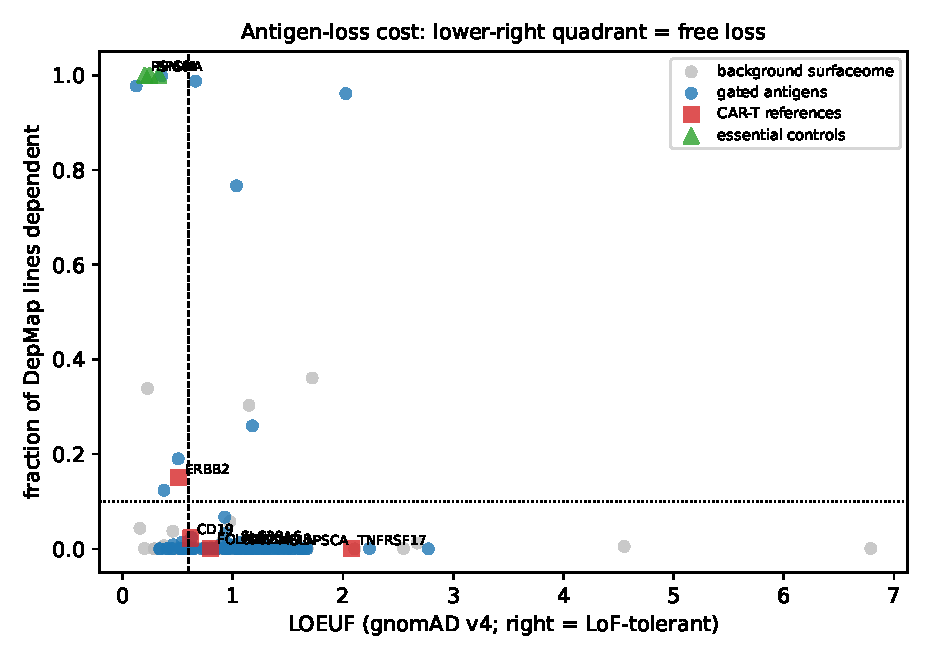
\includegraphics[width=0.8\linewidth]{figs/constraint_escape.pdf}
\caption{Germline LoF tolerance (gnomAD v4 LOEUF, x axis; right of the dashed line at 0.6 = LoF-tolerant) against DepMap 24Q4 dependent-line fraction (y axis; below the dotted line at 0.1 = non-essential). The lower-right quadrant is free antigen loss. Essential controls (green) sit at the opposite corner, validating the axes.}
\end{figure}
\paragraph{Negative results preserved.} None of the three escape-cost axes separates the gated set from background, and LOEUF does not track DepMap dependency across the union (Spearman $\rho=0.07$, $p=0.358$; germline and somatic essentiality are independent axes here).
